\section{Versuchsdurchführung}

\begin{figure}[H]
    \centering
    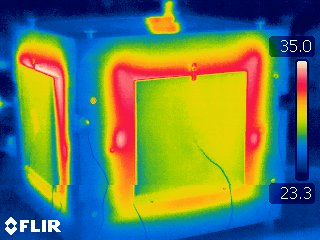
\includegraphics[width=0.9\textwidth]{Abbildungen/WBK_UWERT.jpg}
    \caption{Aufnahmen der Wärmebildkamera des Versuchsaufbaus}
    \label{fig:230715_WBK}
\end{figure}

Zu Beginn des Versuchs werden die Temperaturfühler an die Thermometer angeschlossen und am Modellhaus angebracht. Dabei wird einer an der Außenseite und einer an der Innenseite des Modellhauses befestigt 
um die Außen- und Innenlufttemperatur zu verfolgen. Darauffolgend werden vier unterschiedlichen Wände (Schichtholz unterschiedlicher Dicke, Polystyrol und Glas) mit Temperaturfühlern an Innen- und Au"senseite ausgestattet (im Innern und Außen) und 
das Modellhaus mit dem gedämmten Deckel verschlossen.

\begin{figure}[H]
    \centering
    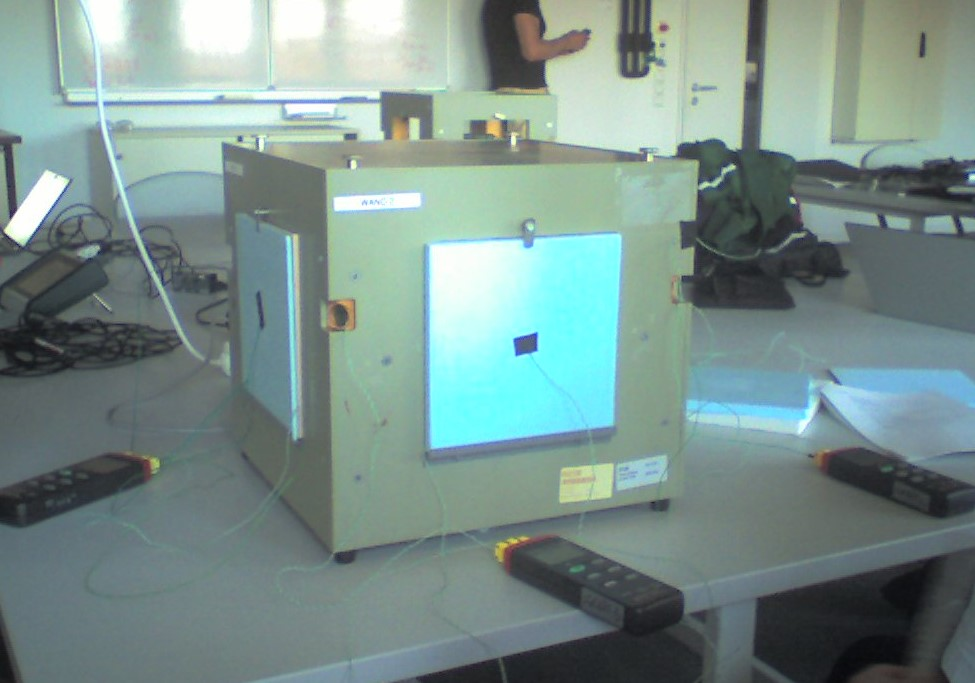
\includegraphics[width=0.9\textwidth]{Abbildungen/M2_Modellhaus.jpeg}
    \caption{Versuchsaufbau der 2. Messreihe}
    \label{fig:230715_M2}
\end{figure}

Die Wärmequelle (Glühlampe), wird in Betrieb genommen und nach Erreichen des stationären Zustandes werden die Temperatur-Messreihen in 30 Sekunden Abständen aufgenommen. Nach 5 Minuten endet die Messreihe.
 Danach werden die beiden Holzwände um Polystyrol beziehungsweise Polystyrol und eine dazwischen liegende Luftschicht erweitert. Im Anschluss werden jeweils erneut Messreihen aufgenommen. 
Abschließend werden mithilfe der Thermografiekamera (\autoref{fig:230715_WBK}) mögliche thermische Schwachstellen ermittelt.